\chapter{Algoritmos evolutivos multiobjetivo basados en descomposición}

En este capítulo, será introducida una nueva clase de algoritmos evolutivos que afrontan la optimización objetivo de una forma diferente a los demás: los algoritmos basados en descomposición. Comenzaremos con uno de los más conocidos: el MOEA/D.

%\section{MOEA/D}
\section{Multiobjective Evolutionary Algorithm based on Decomposition}

\emph{Multiobjective Evolutionary Algorithm based on Decomposition}, o por sus siglas MOEA/D, \cite{zhang2007moea} es un algoritmo evolutivo que emplea el concepto de descomposición para resolver problemas de optimización multiobjetivo. La \emph{descomposición} consiste en asociar cada solución de un conjunto óptimo de Pareto a un problema de optimización escalar\footnote{Por <<problema de optimización escalar>>, endiéndase <<problema de optimización con una única función objetivo>>}, de forma que un frente de Pareto pueda ser \emph{descompuesto} en un cierto número de subproblemas de optimización escalar. Para ello, pueden usarse diferentes funciones de agregación que transformen cada vector de valores objetivo en un valor escalar, las cuales se expondrán con detalle más adelante.

La idea de usar descomposición en un MOEA viene dada por el hecho de que la dominancia de Pareto, como ya se vio previamente en la sección \ref{sec:mop}, no define un orden total entre las soluciones en el espacio objetivo, por lo que resulta más difícil en tal caso seleccionar (o descartar) las soluciones que se generan a lo largo del proceso de búsqueda.

\subsection{Funcionamiento general}

MOEAD/D necesita descomponer el problema de optimización multiobjetivo que se pretende resolver, y para ello necesita una función de agregación $g(\textbf{x})$ que tome como entrada una solución de nuestro problema (o sea, un vector \textbf{x}) y devuelva como salida un valor escalar. De esta forma se puede convertir o \emph{descomponer} el problema de optimización multiobjetivo en un cierto número de subproblemas de optimización escalar.

Para tal fin, la función de agregación necesita de vectores de pesos. Cada uno de ellos consiste en un vector de valores no negativos $\boldsymbol\lambda = (\lambda_1,\dots,\lambda_m)^T$ tal que $\sum_{i=1}^m \lambda_i = 1$, de modo que un subproblema de optimización escalar consistiría en encontrar la solución \textbf{x} que optimice la función de agregación $g(\textbf{x} | \boldsymbol\lambda)$ para un $\boldsymbol\lambda$ dado. De esta forma, por cada vector de pesos, existirá un subproblema de optimización escalar, puesto que para cada vector de pesos $\boldsymbol\lambda$ habrá que encontrar la solución $\textbf{x}^*$ que lo optimice. La notación $g(\textbf{x} | \boldsymbol\lambda)$ hace énfasis en el hecho de que $\boldsymbol\lambda$ es un vector de coeficientes, mientras que $\textbf{x}$ es el vector con las variables que se han de optimizar.

En otras palabras, podría decirse que cada $\boldsymbol\lambda$  representa un subproblema, y que por tanto habrá tantos subproblemas escalares como vectores de pesos. Además, lo ideal es que todos ellos estén lo más uniformemente distribuidos para que todo el frente de Pareto quede bien representado al descomponerse.

En MOEA/D se asume que la función de agregación $g(\textbf{x} | \boldsymbol\lambda)$ es continua, y que si dos vectores de pesos $\boldsymbol\lambda^i$ y $\boldsymbol\lambda^j$ son cercanos, sus respectivas soluciones óptimas de $g(\textbf{x} | \boldsymbol\lambda^i)$ y $g(\textbf{x} | \boldsymbol\lambda^j)$ también serán cercanas. Este hecho es importante, porque ayuda a encontrar el $\textbf{x}^*$ óptimo de un determinado vector $\boldsymbol\lambda^i$ a partir de los $\textbf{x}^*$ óptimos de sus vectores más cercanos. Para sacar provecho de ello, se define para cada $\boldsymbol\lambda^i$ un vecindario $B(i) = \{i_1,\dots,i_T\}$, de forma que el conjunto conformado por los vectores $\{\boldsymbol\lambda^{i_1},\dots,\boldsymbol\lambda^{i_T}\}$ representa los $T$ vectores de pesos más cercanos a $\boldsymbol\lambda^i$. De esta forma, como la población se compone de la mejor solución encontrada hasta el momento para cada subproblema, solo las soluciones actuales son aprovechadas para optimizar cada subproblema escalar usando estos vectores de pesos.

Por último, cabe destacar que, como la población se compone de la mejor solución encontrada hasta el momento para cada subproblema, tendremos tantos individuos \textbf{x} como subproblemas. Dicho de otra forma: a cada \textbf{x} de la población de corresponde un vector de pesos $\boldsymbol\lambda$ que lo optimice.

\begin{figure}
	\centering
	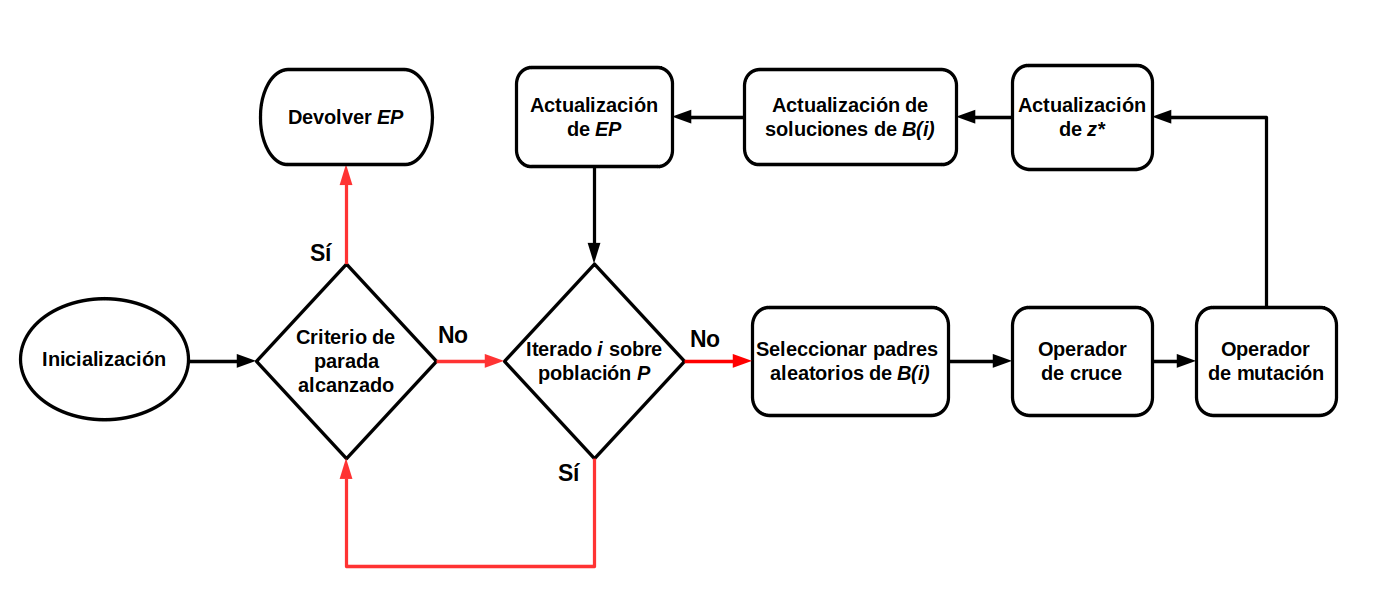
\includegraphics[width=1.1\textwidth]{Images/moead_flowchart}
	\caption{Diagrama de flujo del MOEA/D}
	\label{fig:moeadflow}
\end{figure}

\subsection{Métodos de descomposición}\label{sec:decompmethods}

Las siguientes son algunos métodos de descomposición que pueden emplearse con MOEA/D para generar, por medio de diferentes funciones de agregación, problemas de optimización escalares:

\begin{enumerate}
	\item \textbf{Método de Suma Ponderada} (\emph{Weighted Sum}) .
	
	Sea $\boldsymbol\lambda = \{\lambda_1,\dots,\lambda_m\}$ un vector de pesos no negativos tal que $\sum_{i=1}^m \lambda_i = 1$. La solución óptima para el siguiente problema de optimización:
	
	\begin{equation}
		\max_{\textbf{x} \in \Omega}{~~g^{ws}(\textbf{x} | \boldsymbol\lambda) = \sum^{m}_{i=1} \lambda_i f_i(\textbf{x})}
	\end{equation}
	
	es una solución Pareto-óptima del problema de optimización multiobjetivo a resolver. El conjunto de vectores $\boldsymbol\lambda$ que se utilicen determinará el conjunto de Pareto que se obtenga. Este sencillo enfoque puede resultar útil si el frente de Pareto es convexo (o cóncavo si el problema es de maximización) \cite{miettinen2012nonlinear}.% De lo contrario, es posible que no se encuentren muchas de las soluciones Pareto-óptimas posibles.
	
	\item \textbf{Método de Tchebycheff}.
	
	En este enfoque el problema escalar de optimización es el siguiente:
	
	\begin{equation}\label{eq:tchebycheff}
		\min_{\textbf{x} \in \Omega}{~~g^{te}(\textbf{x} | \boldsymbol\lambda, \textbf{z}^*) = \max_{1 \leq i \leq m}{ \{\lambda_i |f_i(\textbf{x}) - z^*_i|\} }}
	\end{equation}
	
	donde $\textbf{z}^* = (z^*_1,\dots,z^*_m)$ es el punto de referencia o punto ideal, de forma que si nuestro problema es de minimización, entonces $z^*_i = \min_{\textbf{x} \in \Omega}{f_i(\textbf{x})}$. Nótese que se asume que todas las funciones objetivo están acotadas. En caso de no conocer cuál es el punto, puede usarse como aproximación el mínimo de los $f_i(\textbf{x})$ encontrados hasta el momento en el proceso de búsqueda.
	
	Puede demostrarse que el problema de optimización descrito en (\ref{eq:tchebycheff}) siempre tiene al menos una solución óptima, y si esa solución es única, entonces será Pareto-óptima. También se cumple que, para cualquier solución Pareto-óptima $x^*$, siempre existirá un vector de pesos mayores que $0$ para el cual $x^*$ será una solución óptima de (\ref{eq:tchebycheff}) \cite{miettinen2012nonlinear}.
	
	 %La desventaja de este método consiste en que su función de agregación $g^{te}(\textbf{x} | \boldsymbol\lambda, \textbf{z}^*)$ no muestra un comportamiento
	
	\item \textbf{Método de Interseción de Frontera} (\emph{Boundary Intersection}).
	
	
	Normalmente, el frente de Pareto de un problema de optimización objetivo se sitúa en el límite inferior izquierdo o en el límite superior derecho, dependiendo de si el problema es de minimización o maximización respectivamente. Si se dispone de un conjunto de rectas uniformemente distribuidas, los puntos de intersección entre el límite definido por el frente de Pareto y ese conjunto de rectas conforman una buena aproximación del frente de Pareto. Es posible usar este método en MOEA/D usando el punto de referencia $\textbf{z}^*$ y los vectores de pesos $\boldsymbol\lambda$ para construir dichas rectas, de forma que todas las rectas pasen por $\textbf{z}^*$ y tengan como dirección la que determine cada vector $\boldsymbol\lambda$. A partir de ahí, puede generarse el siguiente problema de optimización escalar:
	
	\begin{equation}
	\begin{array}{c}
		\min_{\textbf{x} \in \Omega}{~~g^{bi}(\textbf{x} | \boldsymbol\lambda, \textbf{z}^*) = d} \\
		\text{sujeto a  } ~~F(\textbf{x}) - \textbf{z}^* = d \lambda
		\end{array}.
		\label{eq:bi}
	\end{equation}

	Es preciso aclarar que aquí se asume que el problema de optimización es de minimización. Si, por el contrario, el problema es de maximización, la restricción de igualdad definida en (\ref{eq:bi}) se ha de cambiar por lo siguiente:
	
	
	\begin{equation}
	\textbf{z}^*-F(\textbf{x}) = d \boldsymbol\lambda.
	\end{equation}
	
	  En cualquier caso, esta restricción de igualdad asegura que el vector de valores objetivo $F(\textbf{x})$ siempre se sitúe sobre $L$, la recta con dirección $\boldsymbol\lambda$ (el vector de pesos) y que pasa por el punto $\textbf{z}^*$ (el punto ideal en el espacio objetivo). Esta restricción, sin embargo, resulta difícil de manejar. Para solventar esto, puede utilizarse otro método cuya función de agregación introduzca una penalización, para evitar así la inclusión de restricciones:
	
	\begin{equation}\label{eq:pbi}
		\min_{\textbf{x} \in \Omega}{~~g^{bi}(\textbf{x} | \boldsymbol\lambda, \textbf{z}^*) = d_1 + \theta d_2}
	\end{equation}

	donde, en caso de minimización,
	
	\begin{equation}
	d_1 = \frac{|| (F(\textbf{x}) - \textbf{z}^*)^T \boldsymbol\lambda ||}{||\boldsymbol\lambda||}
	\end{equation}
	\begin{equation}
	d_2 = || F(\textbf{x}) - (\textbf{z}^* + d_1 \boldsymbol\lambda) ||
	\end{equation}
	
	o, si se trata de maximización,

	\begin{equation}
	d_1 = \frac{|| (\textbf{z}^* - F(\textbf{x}))^T \boldsymbol\lambda ||}{||\boldsymbol\lambda||}
	\end{equation}
	
	\begin{equation}d_2 = || F(\textbf{x}) - (\textbf{z}^* - d_1 \boldsymbol\lambda) ||
	\end{equation}
	
	Geométricamente, $d_1$ representa la distancia entre $z^*$ y la proyección de $F(x)$ sobre la recta $L$, mientras que $d_2$ es la distancia entre $F(x)$ y la recta $L$, es decir, la distancia entre  $F(x)$ y su proyección en $L$. Nótese que aquí $d_1$ es el equivalente a $d$ en la expresión \ref{eq:bi}, y $d_2$ es el valor que representa. Por su parte, $\theta > 0$ es un parámetro de penalización que determina cómo de importante es que se minimice $d_2$. Si dicho parámetro $\theta$ es ajustado adecuadamente, las soluciones de ambos métodos (\ref{eq:bi}) y (\ref{eq:pbi}) serán muy similares.
	
	En \cite{zhang2007moea}, este método recibe el nombre de Método de Intersección de Frontera Basado en Penalización o PBI (\emph{Penalty-based Boundary Intersection Method}). Su principal ventaja frente al enfoque de Tchebycheff es que se obtienen soluciones más uniformemente distribuidas, para el mismo conjunto de vectores de pesos. Además, para dos soluciones $\textbf{x}$ e $\textbf{y}$ tales que $\textbf{x} \preceq \textbf{y}$, con el método de Tchebycheff es posible que ocurra que $g^{te}(\textbf{x} | \boldsymbol\lambda, \textbf{z}^*) = g^{te}(\textbf{y} | \boldsymbol\lambda, \textbf{z}^*)$, mientras que es difícil que pase lo mismo con PBI.
	
\begin{figure}[H]
	\centering
	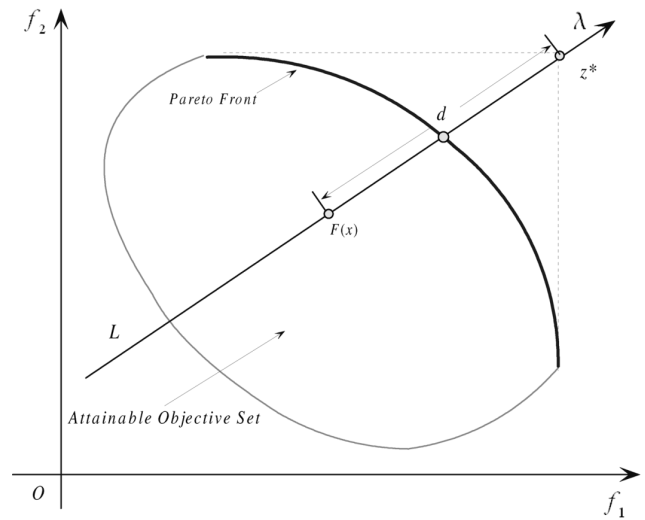
\includegraphics[width=1.0\textwidth]{Images/bi}
	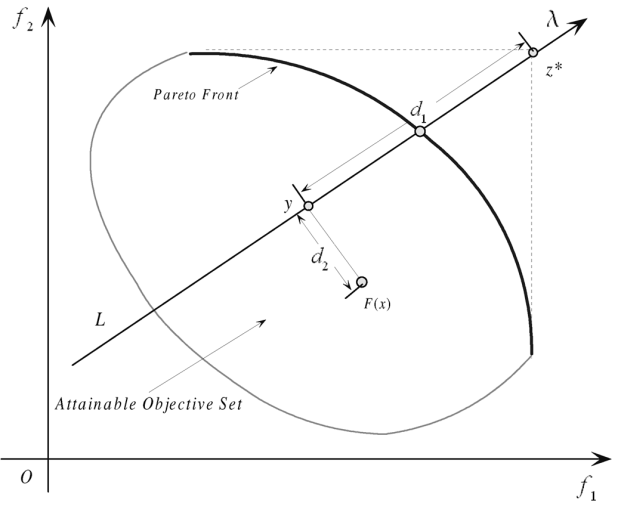
\includegraphics[width=1.0\textwidth]{Images/pbi}
	\caption[Ilustración geométrica de los métodos BI y PBI para un problema de maximización.]{Ilustración geométrica de los métodos BI (arriba) y PBI (abajo) para un problema de maximización \cite{zhang2007moea}.}
	\label{fig:boundaryint}
\end{figure}
	
	Sin embargo, el principal inconveniente del método PBI es el hecho de que $\theta$ sea un parámetro, y como tal debe ser ajustado adecuadamente. Un valor demasiado bajo o demasiado alto provocará que los resultados empeoren.

\end{enumerate}
\newpage



\begin{algorithm}[h]
	\LinesNumbered
	\BlankLine
	\KwIn{Número de subproblemas $N$, tamaño del vecindario de los vectores de pesos $T$, opcionalmente conjunto de vectores de pesos uniformemente distribuidos $\{\lambda_1,\dots,\lambda_N\}$}
	\BlankLine

	\tcc{Inicialización}
	Inicializar población externa $EP = \emptyset$\\
	
	Generar conjunto de vectores de pesos uniformemente distribuidos $\{\lambda_1,\dots,\lambda_N\}$ (si no se ha pasado como entrada)\\
	
	Calcular distancia euclídea entre todos los pares de vectores de pesos. Hayar $B(i) = \{i_1,\dots,i_T\}$ para todo $i\in\{1,\dots,N\}$, de forma que $\boldsymbol\lambda^{i_1},\dots,\boldsymbol\lambda^{i_T}$ son los $T$ vectores más cercanos a $\boldsymbol\lambda^{i}$ \\
	Inicializar, aleatoriamente o de otra forma, la población $P$\\
	
	Obtener valores objetivos de la población $FV$:~~$FV^i = F(\textbf{x}^i)$ para todo $i\in\{1,\dots,N\}$\\
	\BlankLine
	
	\tcc{Actualización}
	\While{criterio de parada no se cumple}{

		\For{$i\in\{1,\dots,N\}$}{
			Elegir aleatoriamente dos valores $l,k \in B(i)$\\
			Generar un descendiente $\textbf{y}$ aplicando el operador de cruce sobre $\textbf{x}^l$ y $\textbf{x}^k$\\
			Aplicar sobre $\textbf{y}$ el operador de mutación. Aplicar opcionalmente mejora o reparación.\\
			
			\BlankLine
			\tcc{Actualizar punto ideal $z$}
			\For{$j\in\{1,\dots,m\}$}{
				
				\If{$f_j(\textbf{y}) \leq z_j$}{
					$z_j = f_j(\textbf{y})$
				}
			}
			\BlankLine
			\tcc{Actualizar soluciones vecinas}
			\For{$j\in B(i)$}{
				\If{$g(\textbf{y} | \boldsymbol\lambda^j) \leq g(\textbf{x}^j | \boldsymbol\lambda^j)$}{
					$\textbf{x}^j = \textbf{y}$,~~~$FV_j = F(\textbf{y})$
				}
			}
			
			\BlankLine
			\tcc{Actualizar población externa}
			Eliminar de $EP$ todas las soluciones dominadas por $F(\textbf{y})$\\
			Añadir $F(\textbf{y})$ a $EP$ si ningún vector de $EP$ domina a $F(\textbf{y})$
		}
	}
	\BlankLine
	
	\KwRet $EP$

	\BlankLine
	\caption{MOEA/D}
	\label{alg:moead}
\end{algorithm}


\section{El framework ADA}

En este apartado se introducirá el esquema usado en este trabajo que introduce el manejo de la multimodalidad en los algoritmos evolutivos multiobjetivo basados en descomposición. Antes de eso, para poner al lector en situación, se hablará brevemente sobre el concepto de multimodalidad y su relación con los MOEAs.

\subsection{Algoritmos evolutivos multimodales multiobjetivo basados en descomposición}

En muchos MOEAs se asume que únicamente la distribución de las soluciones en el espacio objetivo es relevante, dejando en un segundo plano la diversidad en el espacio de soluciones. Sin ir más lejos, un buen ejemplo de esto es el propio MOEA/D, con el cual se puede mantener una buena diversidad en el espacio objetivo si se escoge un método de descomposición adecuado y, sobretodo, si se emplea un conjunto de vectores de pesos que estén uniformemente bien distribuidos \cite{zhang2007moea}. Sin embargo, no existe en MOEA/D ningún mecanismo que mantenga la diversidad en el espacio de soluciones.

Pueden darse situaciones en las que existan diversas soluciones que, aún siendo muy distantes en el espacio de soluciones, son muy próximas o similares en el espacio objetivo, como puede apreciarse en la figura \ref{fig:multimodal}, que ilustra a la perfección el concepto de \emph{multimodalidad}. El hecho de que en un problema existan formas muy distintas de llegar a (casi) la misma solución es algo muy relevante, pues permite elegir entre distintas soluciones de una calidad similar en función de un cierto criterio o preferencia (por ejemplo, que alguna solución sea más fácil de obtener, que una se las soluciones se vuelva inalcanzable o totalmente inviable, etc). Por ello, en ciertos problemas es importante mantener la diversidad en el espacio de soluciones.

Los llamados algoritmos evolutivos multimodales multiobjetivo son MOEAs pensados para problemas en los que se dan precisamente estas circunstancias, los llamados problemas de optimización multiobjetivo multimodales. Su objetivo consiste en encontrar el mayor número de soluciones Pareto-óptimas equivalentes, para lo cual se sirven de mecanismos para manejar múltiples soluciones equivalentes durante su ejecución. Algunos ejemplos de este tipo de algoritmos son el $P_{Q,\epsilon}$-MOEA, el Omni-optimizer y el DIOP, entre otros.


\subsection{ADA: un framework para manejar la multimodalidad}

ADA \cite{tanabe2019framework} es un método propuesto en 2019 para manejar la multimodalidad en los MOEAs basados en descomposición. No se trata de un algoritmo en sí, sino que es un \emph{framework}, es decir, un esquema o marco general que puede aplicarse a distintos algoritmos.

ADA es una generalización de MOEA/D-AD \cite{tanabe2018decomposition}, una versión del MOEA/D capaz de manejar la multimodalidad propuesta por los mismos autores de ADA, con un mecanismo para mantener la diversidad en el espacio basado en el concepto de vecindario de soluciones. Lo cierto es que MOEA/D-AD no es una adaptación trivial del MOEA/D básico, sino que cambia por completo su diseño y funcionamiento.



\subsection{Operadores de ADA}

MOEA/D-AD posee distintos componentes y operadores, cada uno de los cuales cumple un papel fundamental. De hecho, el nombre de MOEA/D-AD viene de MOEA/D \emph{Adition-Deletion}, haciendo alusión a dos de sus componentes: sus operadores de adición y eliminación, respectivamente. ADA posee esos mismos operadores, con la diferencia de que los operadores de MOEA/D-AD son de una forma determinada, mientras que en ADA pueden adoptar distintas formas y variantes, dependiendo de sobre qué algoritmo se esté aplicando.

\subsubsection{Operadores genéticos y de selección}

Como todo algoritmo evolutivo, ADA hace uso de operadores de cruce y mutación para generar nuevas soluciones a partir de las ya existentes. Al igual que en MOEA/D, con ADA puede usarse cualquier operador de cruce clásico, como el operador uniforme o el operador de punto fijo, en caso de usar un esquema de codificación binaria o entera para los cromosomas/individuos de la población, u operadores de cruce como el BLX-$\alpha$ \cite{eshelman1993real} o el SBX \cite{deb1995simulated}, si se usa codificación real. Por supuesto, también pueden usarse operadores de cruce para problemas específicos.

Por su parte, el método de selección de padres de ADA y MOEA/D-AD es de lo más sencillo: mientras que en el MOEA/D original se seleccionaban dos individuos cuyos respectivos vectores de pesos estuviesen en el vecindario del individuo actual $\textbf{x}^i$ (ver líneas 6 y 7 del algoritmo \ref{alg:moead}), en ADA y MOEA/D-AD simplemente se seleccionan dos padres aleatorios de toda la población $P$.

\begin{figure}
	\centering
	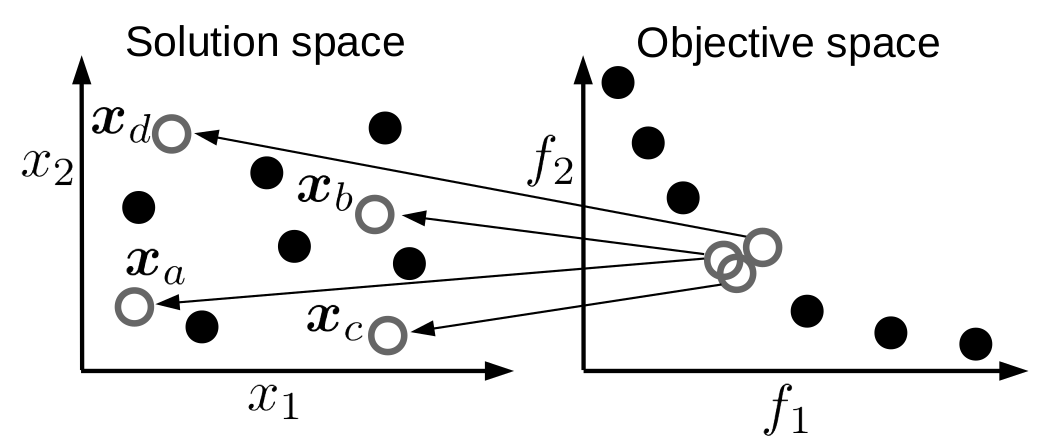
\includegraphics[width=1.0\textwidth]{Images/multimodal}
	\caption[Ilustración del concepto de multimodalidad, en la cual soluciones muy dispares en el espacio de soluciones son casi idénticas en el espacio objetivo.]{Ilustración del concepto de multimodalidad, en la cual soluciones muy dispares en el espacio de soluciones son casi idénticas en el espacio objetivo.\cite{tanabe2019framework}}
	\label{fig:multimodal}
\end{figure}

\subsubsection{Operador de asignación}

En MOEA/D, desde el principio habrá uno y solo un individuo asignado a cada vector de pesos $\boldsymbol\lambda$ (cada uno de los cuales representaba un subproblema), de forma que al individuo $\textbf{x}^i$ le corresponde el subproblema dado por $\boldsymbol\lambda^i$. A lo largo de toda la ejecución, tanto el número de individuos en la población como el número de vectores de pesos se mantiene fijo en $N$, optimizando cada individuo de acuerdo a su correspondiente vector de pesos.

En ADA y MOEA/D-AD no ocurre lo mismo. Mientras que sí se mantienen siempre los mismos vectores de pesos , el tamaño de la población de individuos va cambiando a lo largo del proceso de búsqueda. Además, la forma en la que se asignan las soluciones a los vectores de pesos es diferente: no tiene por qué asignarse el $i$-ésimo individuo $\textbf{x}^i$ al $i$-ésimo vector $\boldsymbol\lambda^i$, si no que ahora $\textbf{x}^i$ se asigna al $j$-ésimo vector $\boldsymbol\lambda^j$, siendo $\boldsymbol\lambda^j$ el vector de pesos que mejor se adapta a $\textbf{x}_i$  bajo un cierto criterio.

Es necesario mantener una estructura que permita saber a qué vector de pesos se ha asignado la solución $\textbf{x}^i$. Así pues, se define el vector $\textbf{a} = (a_1,\dots,a_\mu)$, donde $\mu=|P|$ (recordemos que en ADA y en MOEA/D-AD el tamaño de la población es variable), de forma que si $a_i = j$ entonces al individuo $\textbf{x}^i$ le corresponde el vector $\boldsymbol\lambda^{j}$, y por tanto habrá sido asignado al $j$-ésimo subproblema escalar.

El criterio para asignar individuos a vectores de pesos puede basarse en uno de los métodos de descomposición descritos en la sección \ref{sec:decompmethods}. Si, por ejemplo, se usase el enfoque de Tchebycheff, una solución $\textbf{x}$ se asignaría al $j$-ésimo subproblema, donde:

\begin{equation}
 j = \argmin_{k\in\{1,\dots,N\}}\{g^{te}(\textbf{x}|\boldsymbol\lambda^k)\}
\end{equation}

En MOEA/D-AD, por su parte, se emplea la distancia perpendicular entre el vector normalizado de valores objetivos $F(\textbf{x})$ de una solución $\textbf{x}$, y un vector de pesos $\boldsymbol\lambda$, que no es sino la distancia entre $F(\textbf{x})$ normalizado y su proyección en la recta que pasa por el punto referencia $\textbf{z}$ con la dirección determinada por $\boldsymbol\lambda$ (véase el valor $d_2$ de la fórmula \ref{eq:pbi}).


\subsubsection{Criterio de vecindario}\label{sec:neigh}

Tanto en MOEA/D como en MOEA/D-AD y las variantes de ADA, la diversidad en el espacio objetivo se mantiene mediante la asignación de individuos (soluciones) a los diferentes subproblemas, descrita justo en el apartado anterior. Sin embargo, en lo que se refiere al espacio de soluciones, ningún mecanismo para mantener la diversidad en el espacio de soluciones se emplea en MOEA/D, mientras que en MOEA/D-AD y ADA sí.

La forma de controlar la diversidad en el espacio de soluciones consiste en un criterio de vecindad. Para ello, en \cite{tanabe2019framework} y \cite{tanabe2018decomposition} se propone usar la distancia Euclídea entre soluciones, habiendo normalizado antes las variables de decisión (cromosomas) si en ellas se emplean distintas escalas de valores. De esta forma, puede determinarse para cada solución un vecindario conformado por las $L$ soluciones más cercanas.

Además de este sencillo criterio basado en distancias, con ADA puede usarse cualquier otro criterio de vecindad o de nichos, pero en el estudio preliminar llevado a cabo en \cite{tanabe2019framework} se vió que otros criterios más sofisticados no funcionarion bien.



\subsubsection{Operador de eliminación}

En ADA, el criterio según el cual se descartan las soluciones de la población $P$ es clave, pues ha sido ideado teniendo en mente  la diversidad tanto del espacio de soluciones como la del espacio objetivo.

Sea $\textbf{u}$ una nueva solución generada a partir de dos soluciones padres mediante los operadores genéticos. Se construyen dos conjuntos de soluciones a partir de $\textbf{u}$, a los que llamaremos $Y$ y $Z$, definidos de la siguiente forma:
\begin{equation}
	\begin{array}{c}
		Y = \{ \textbf{x} \in P ~|~ \text{\textbf{x} es vecino de \textbf{u} en el espacio de soluciones} \} \\ 
		Z = \{ \textbf{x} \in P ~|~ \text{\textbf{x} está asignado al mismo subproblema que \textbf{u}} \}
	\end{array}.
\end{equation}


El conjunto $Y$ se basa en el criterio de vecindario que se haya escogido, del cual se habla en el anterior apartado, mientras que $Z$ se basa en el operador de asignación. A partir de estos dos conjuntos, se construye uno tercero, al que llamamos $X$, compuesto por las soluciones que cumplen tanto la condición de $Y$ como la de $Z$: 

\begin{equation}
	X = Y \cap Z
\end{equation}

Posteriormente, se compara la nueva solución $\textbf{u}$ con cada una de las soluciones de $X$. Aquellas soluciones de $X$ que sean peores que $\textbf{u}$ según un cierto criterio serán eliminadas de la población $P$.

¿Por qué se comparan con $\textbf{u}$ solo las soluciones de $X$, y no con las de $Y$ y luego con las de $Z$ por separado? Supongamos que, en un momento dado durante la ejecución de ADA, existe una solución $\textbf{x}'$ tal que $\textbf{x}' \in Z$ y $\textbf{x}' \not\in Y$. Si resultase que $\textbf{x}'$ fuese peor que $\textbf{u}$ y se eliminase de la población $P$, estaríamos perdiendo una solución que aporta diversidad al espacio de soluciónes, ya que $\textbf{u}$ no pertenece al vecindario de $\textbf{u}$. De forma análoga, si $\textbf{x}' \in Y$ pero $\textbf{x}' \not\in Z$, eliminar a $\textbf{x}'$ tampoco tendría sentido aunque fuese, de alguna forma, peor que $\textbf{u}$, porque ni siquiera está asignado al mismo subproblema que $\textbf{u}$, por lo que se perdería una solución que aporta diversidad al espacio objetivo. Por lo tanto, solo eliminando soluciones que pertenezcan a $X$ es posible asegurarse de que no se pierde diversidad ni en el espacio de soluciones ni en el espacio objetivo, porque así se eliminan únicamente soluciones que sean vecinas de $\textbf{u}$ (cercanas a $\textbf{u}$ en espacio de soluciones) y que al mismo tiempo estén asignadas al mismo subproblema que $\textbf{u}$ (cercanas a $\textbf{u}$ en espacio objetivo).

En ADA pueden usarse distintos criterios para determinar si una solución es peor que otra. Si se aplica ADA en algún algoritmo basado en MOEA/D, como el MOEA/D-AGR \cite{wang2015adaptive}, puede usarse cualquiera de los métodos de descomposición listados en la sección \ref{sec:decompmethods}. Si, por ejemplo, se optase por usar el enfoque de Tchebycheff, entonces una solución $\textbf{x}$ sería peor que otra solución $\textbf{y}$ si y solo si $g^{te}(\textbf{y} | \boldsymbol\lambda, \textbf{z}^*) \leq g^{te}(\textbf{x} | \boldsymbol\lambda, \textbf{z}^*)$ para el mismo vector de pesos $\boldsymbol\lambda$. 

\begin{figure}
	\centering
	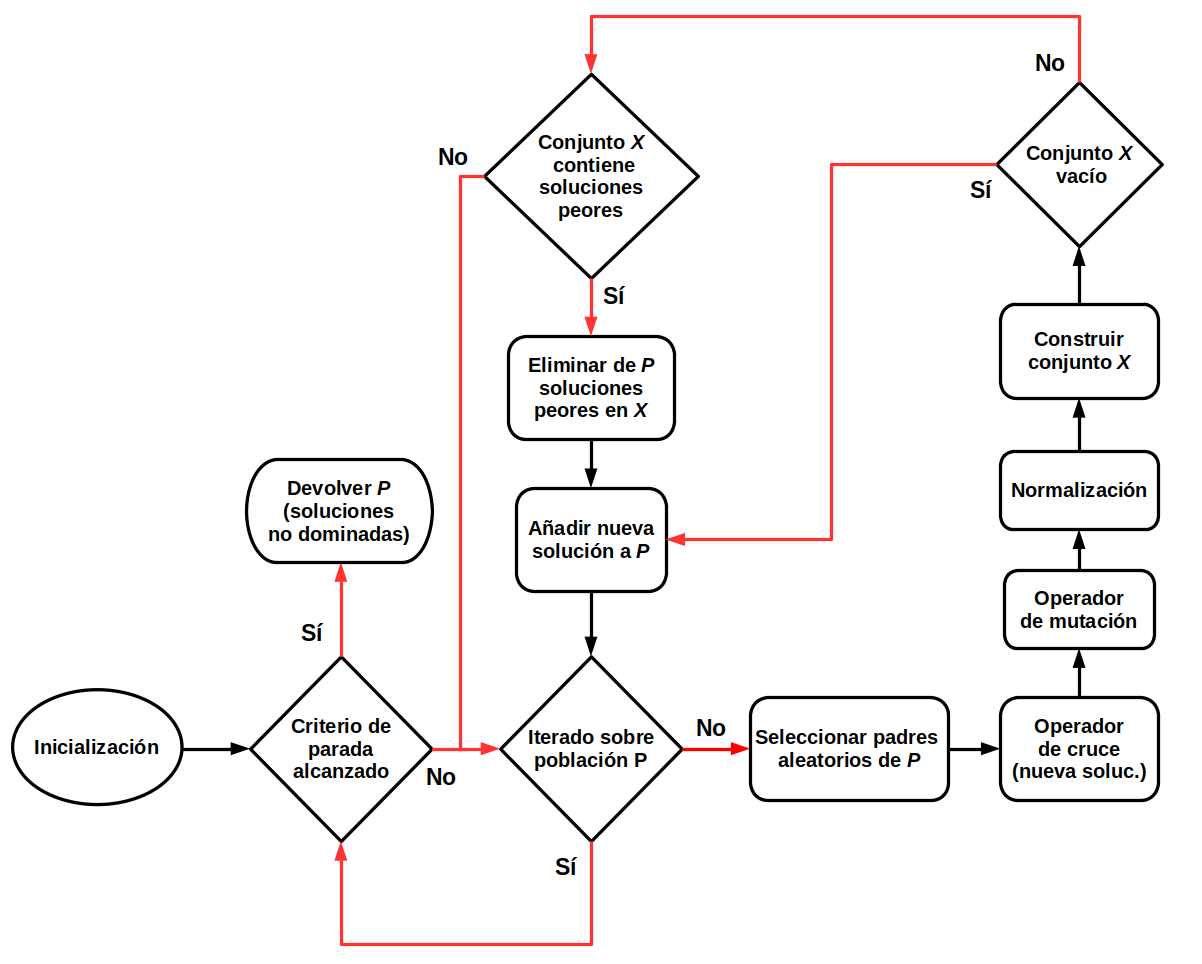
\includegraphics[width=1.1\textwidth]{Images/moead_ada_flowchart}
	\caption{Diagrama de flujo del esquema ADA}
	\label{fig:adaflow}
\end{figure}

\subsubsection{Operador de adición}

Una vez comparada la nueva solución $\textbf{u}$ con todas las soluciones del conjunto $X$ (si las hubiese), y eliminadas aquellas que fuesen peores, llega el momento de decidir qué hacer con $\textbf{u}$: si añadirla a la población $P$ o descartarla. De esto se encargará el operador de adición, el cual añadirá $\textbf{u}$ a la población $P$ si se cumple una de estas dos condiciones:
\begin{enumerate}
	\item Si el conjunto $X$ generado a partir de $\textbf{u}$ no tiene elementos\\($X = \emptyset$).
	\item Si $X$ sí tiene elementos, pero al menos uno de ellos es peor\\que $\textbf{u}$.
\end{enumerate}

¿Por qué se añade $\textbf{u}$ si $X = \emptyset$? Si $X$ no tiene elementos, entonces no existen soluciones en $P$ que sean vecinas de $\textbf{u}$ en el espacio de soluciones y que al mismo tiempo estén asignadas al mismo subproblema (puede que existan soluciones que cumplan una condición u otra, pero no ambas a la vez, ya que en tal caso formarían parte de $X$). Por tanto, $\textbf{u}$ es una solución que aporta diversidad, ya sea al espacio de soluciones, al espacio objetivo, o a ambos, por lo que tiene sentido añadirla a la población $P$ aunque esta ya contenga soluciones que sean mejores que $\textbf{u}$.

\begin{figure}[h]
	\centering
	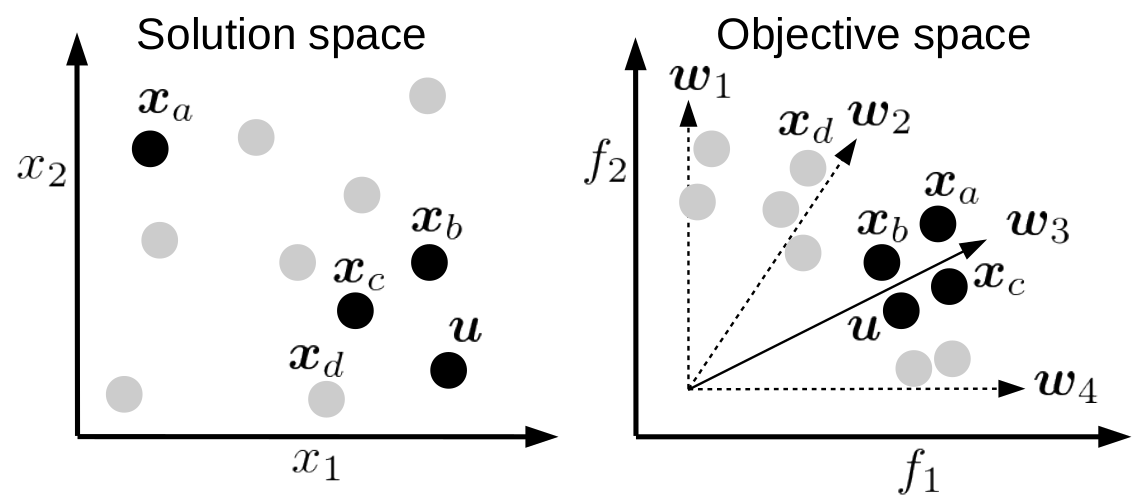
\includegraphics[width=1.0\textwidth]{Images/same_subproblem}
	\caption[Ejemplo que ilustra cómo las soluciones asignadas al mismo subproblema/vector de pesos son cercanas entre sí en el espacio objetivo.]{Ejemplo que ilustra cómo las soluciones asignadas al mismo subproblema/vector de pesos son cercanas entre sí en el espacio objetivo. \cite{tanabe2019framework}}
	\label{fig:assigsubproblem}
\end{figure}


¿Por qué, si $X \not = \emptyset$, $\textbf{u}$ se añade solo si alguna de las soluciones de $X$ es peor que $\textbf{u}$? Porque al ser vecinas de $\textbf{u}$ y estar asignadas al mismo subproblema, no se perderá diversidad si son sustituidas por $\textbf{u}$. Por tanto, si se han eliminado de $P$ soluciones que formaban parte de $X$ por ser peores que $\textbf{u}$, lo lógico es añadir a la propia $\textbf{u}$ a $P$ para reemplazarlas.



\newpage

\begin{algorithm}
	\LinesNumbered
	\BlankLine
	\KwIn{Número de subproblemas $N$, proporción de vecindario $\tau$}
	\BlankLine
	\tcc{Inicialización}
	Inicializar población externa $EP = \emptyset$\\
	
	Generar conjunto de vectores de pesos $\{\lambda_1,\dots,\lambda_N\}$\\
	
	Inicializar, aleatoriamente o de otra forma, la población $P$\\
	
	Obtener $FV$:~~$FV^i = F(\textbf{x}^i)$ para todo $i\in\{1,\dots,N\}$\\
	
	Inicializar problemas asignados $\textbf{a} = (a_1, \dots, a_N)$
	
	\tcc{Op. Asignación}
	\For{$i\in\{1,\dots,N\}$}{
		Encontrar $j$-ésimo subproblema que mejor se adapte a $\textbf{x}^i$\\
		$a_i = j$\\
	}
	\While{criterio de parada no se cumple}{
		\tcc{Tamaño de población y vecindario}
		$\mu = |P|$,  $T = \mu \cdot \tau$\\
		
		\BlankLine
		\tcc{Selección de padres y op. genéticos}
		Seleccionar dos valores aleatorios $a,b \in \{1,\dots,\mu\}$ \\
		Generar un descendiente $\textbf{u}$ aplicando el operador de cruce sobre $\textbf{x}^a$ y $\textbf{x}^b$\\
		\BlankLine
		Aplicar sobre $\textbf{u}$ el operador de mutación. Aplicar opcionalmente mejora o reparación.\\
		Normalizar los vectores de valores objetivos $F(\textbf{u})$ y $FV$\\
		Encontrar $j$-ésimo subproblema que mejor se adapte a $\textbf{u}$\\
		Generar vecindario de $\textbf{u}$ ($T$ soluciones más cercanas)
		$X = \{\textbf{x} \in P ~|~ \textbf{x} \text{ está asignado al subproblema } j \land \textbf{x} \text{ está en el vecindario de \textbf{u}} \}$
		\BlankLine
		% SEPARAR AQUÍ
		\tcc{Op. Eliminación}
		$b^{\text{ ganador}} = FALSE$\\
		$b^{\text{ explorador}} = FALSE$\\
		
		\If{$X = \emptyset$}{
			$b^{\text{ explorador}} = TRUE$\\
		}
		
		\For{$\textbf{x} \in X$}{
			\If{$\textbf{x}$ es peor que $\textbf{u}$}{
					$P = P \setminus \{\textbf{x}\}$\\
					$b^{\text{ ganador}} = TRUE$\\
				}
		}
		
		\BlankLine
		\tcc{Op. Adición}
		\If{$b^{\text{ explorador}} \lor b^{\text{ ganador}}$}{
			$P = P \cup \{\textbf{u}\}$\\
			Añadir $j$ al final de $\textbf{a}$\\
		}
		
	}
	\BlankLine
	\KwRet $P$
	\BlankLine
	\caption{El framework ADA}
	\label{alg:ada}
\end{algorithm}
\newpage




 
 \begin{algorithm}
	\LinesNumbered
	\BlankLine
	\KwIn{Número de subproblemas $N$, tamaño del vecindario de los vectores de pesos $T$, opcionalmente conjunto de vectores de pesos uniformemente distribuidos $\{\lambda_1,\dots,\lambda_N\}$}
	\KwOut{Población externa $EP$}
	\BlankLine
	Adicion\\
	Eliminacion
	\BlankLine
	
	\KwRet $EP$

	\BlankLine
	\caption{MOEA/D-AD}
	\label{alg:moeadad}
\end{algorithm}

